\documentclass[tikz,border=3mm]{standalone}
\usetikzlibrary{positioning,arrows.meta,quotes,decorations.pathmorphing, calc}

\newcommand{\X}{\mathcal{X}}
\newcommand{\ev}{\text{ev}}

\begin{document}
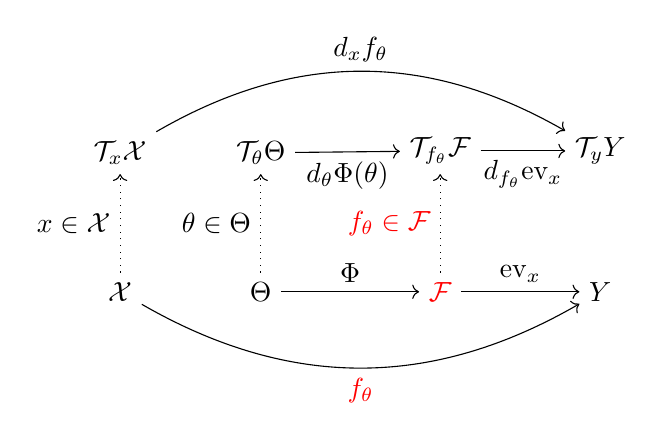
\begin{tikzpicture}[scale=1.0]
\node (X) at (0,0) {\(\X\)};
\node (Theta) [right=1.25cm of X] {$\Theta$};
\node (F) [right=1.75cm of Theta] {$\color{red}{\mathcal{F}}$};
\node (Y) [right=1.5cm of F] {$Y$};
\node (TX) [above=1.25cm of X] {$\mathcal{T}_{x} \X$};
\node (TTheta) [above=1.25cm of Theta] {$\mathcal{T}_{\theta} \Theta$};
\node (TF) [above=1.25cm of F] {$\mathcal{T}_{f_\theta} \mathcal{F}$};
\node (TY) [above=1.25cm of Y] {$\mathcal{T}_{y} Y$};
\draw[->] (Theta) to node[above] {$\Phi$} (F);
\draw[->] (TTheta) to node[below] {$d_\theta \Phi(\theta)$} (TF);
\draw[->, dotted] (Theta) to node[left] {$\theta \in \Theta$} (TTheta);
\draw[->, dotted] (F) to node[left] {$\color{red}{f_\theta \in \mathcal{F}}$} (TF);
\draw[->] (F) to node[above] {ev$_x$} (Y);
\draw[->] (TF) to node[below] {$d_{f_\theta}$ev$_x$} (TY);
\draw[->] (X) to[bend right=30] node[below] {\color{red}{\(f_\theta\)}} (Y);
\draw[->,dotted] (X) to node[left] {$x \in \mathcal{X}$} (TX);
\draw[->] (TX) to[bend left=30] node[above] {\(d_x f_\theta\)} (TY);
\end{tikzpicture}

\end{document}